\chapter{Introduction}

Our universe's origin has always been a mystery until humankind started looking for answers to the unanswered questions about the evolution of the cosmos. The search for solutions led to a field of study called cosmology. This field has drastically impacted our knowledge of the universe's evolution~\citep{book:909085}.

Humans initially believed that the Sun, the moon, and other planets orbited the Earth until Nicolaus Copernicus and other astronomers replaced the geocentric model with the heliocentric model~\citep{sep-copernicus, kanas}.  Celestial mechanics emerged as an area of study after Isaac Newton discovered that elliptical planet motion could be explained by gravitational force attraction~\citep{crowe2013theories,sep-copernicus}. In the modern study of the universe, our understanding of gravity has been further refined by Albert Einstein's theory of general relativity, which presents the mathematical framework required to describe the universe's evolution. The latest observations show that the universe's expansion is accelerating, and the speeds of distant galaxies and their distances from Earth are proved to be directly related. It is assumed that the cosmic microwave background (CMB) is residual radiation from the time the universe began. \attention{[The two observations that cemented the big bang model were the expansion of the universe (not the acceleration, which is outside of the standard big bang framework) and the detection of the CMB.  Remove the mention of acceleration here, and introduce the CMB as a detection, rather than an assumption.]}

As a result of all these findings, Georges Lemaitre proposed the Big Bang theory, the contemporary model that \st{provides a complete explanation of} \attention{explains} the universe's expansion~\citep{1926ApJ....64..321H}. The Big Bang theory was established from Hubble's law and subsequently by Arno Penzias and Robert Wilson in 1964 from discovering the cosmic microwave background (CMB)~\citep{1965ApJ...142..419P, 2003RvMP...75..559P, 1929PNAS...15..168H}. The Supernova Cosmology Project and the High-Z Supernovae Search Team in 1998 discovered the universe's acceleration using observations of type Ia supernovae~\citep{1998AJ....116.1009R, 1999ApJ...517..565P}. The accelerated expansion is described by dark energy, which accounts for approximately 74 percent of the universe's energy density. Today, understanding dark energy's nature is a significant area of focus in astrophysics and particle physics~\citep{2008ARA&A..46..385F}. 

\section{History of the Universe}

\autoref{Fig:timeline} shows the cosmic history of the universe. The Planck era, which lasted until \SI{e-43}{s} after the big bang, is unknown to physicists and requires a quantum theory of gravity. Following the Planck era, \SI{e-34}{s} after the big bang, the universe went through a period of rapid exponential expansion, known as Inflation~\citep{1981PhRvD..23..347G}.

\begin{figure}
	\begin{center}
		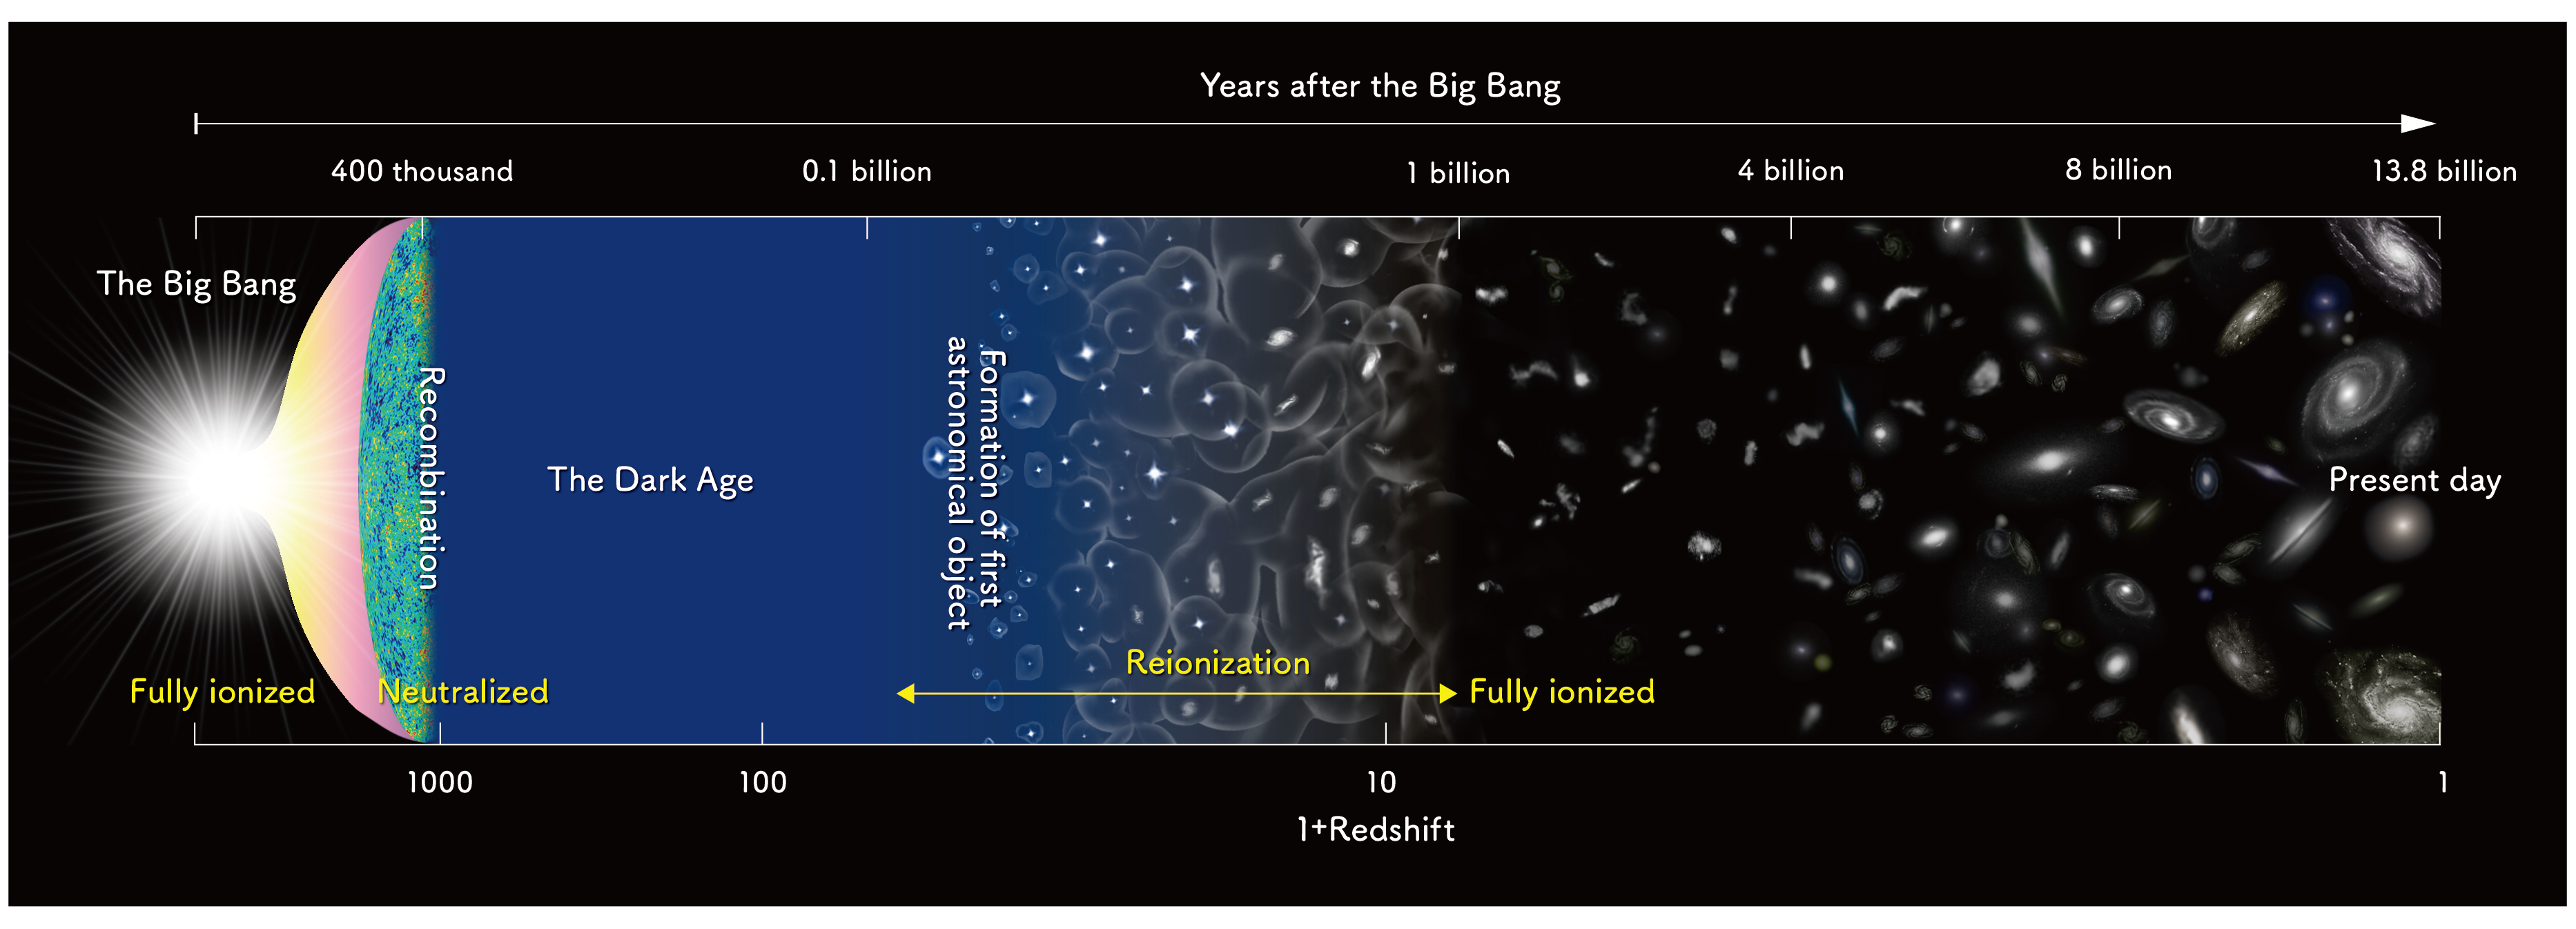
\includegraphics[width=\linewidth]{Figures/Reionizationtimeline.jpg}
		\caption{The cosmic history of the Universe from the Big Bang to its early years, through the dark ages to the epoch of reionization and the post-reionization epoch. Image credit:National Optical Astronomy Observatory}
		\label{Fig:timeline}
	\end{center}
\end{figure} 

Recombination occurred when the universe cooled enough for neutral hydrogen (HI) to form, around a redshift of $z$ $\sim1100$. Redshift enables us to gain access to the early age of the universe, which means that the higher the redshift, the further away we can look back in time. The redshift-wavelength relation is given by
\begin{equation}
\begin{split}
1+z & = \frac{\lambda_{obs}}{\lambda_{emit}}= \frac{1}{a}
\end{split}
\end{equation}
where $z$ is the redshift, $\lambda_{obs}$ is the wavelength of the observed signal, $\lambda_{emit}$ is the wavelength of the signal emitted, and $a$ is the Universe expansion scale factor. Before recombination, electrons were not bound to protons, and the universe contained ionized plasma known as photon-baryon fluid. Decoupled photons then formed the CMB~\citep{1965ApJ...142..419P}.

Subsequently, HI became the dominant baryonic component of the intergalactic medium (IGM) during the dark ages ($1100 \gtrsim z \gtrsim 30$). No measurements of the dark ages exist, and if hydrogen can be mapped in this era, valuable cosmological data can be produced~\citep{11, 2004PhRvL..92u1301L}.

There were density fluctuations in the distribution of matter, and the overdense regions collapsed under the influence of gravity, ultimately creating the first stars\st{. Thus, nuclear reaction resulted} \attention{and resulting} in Cosmic Dawn ($30\gtrsim z \gtrsim 10$). Energy from the first stars ultimately fully reionized the universe. Galaxies, galaxy clusters, and large-scale structures that exist in the present universe evolved after the first stars were born~\citep{2017arXiv170808521D, 2012AdSpR..49..433B}. 

Throughout the cosmological epochs, what is known is minimal because it is challenging to observe them directly. The growth of \SI{21}{cm} cosmology can fill the gaps in our knowledge of the universe's history~\citep{2012RPPh...75h6901P}. A brief overview of the universe's history has been given, and the next section will cover 21 cm cosmology corresponding to the dark ages and cosmic dawn in more detail.

\section{Cosmology with Redshifted 21-cm Emission}

Because hydrogen gas is the most abundant element in the universe, there is a concerted effort in the experimental community to develop telescopes for mapping neutral hydrogen via \SI{21}{cm} emission. This hydrogen line is an essential mechanism for probing the dark ages to the epoch of reionization (EoR)~\citep{2013PhRvD..87d3002L,2014ApJ...782...66P}. The generation of the hydrogen line (\SI{21}{cm} line or HI line) is due to the intrinsic electron and proton spins within the hydrogen atoms~\citep{book:832129}. The electron and proton spins can be oriented in either the opposing or the same direction, respective to each other. When the spins are opposing or antiparallel, the hydrogen atom is in the lower energy state. When the spins are parallel, the hydrogen atom is in a higher energy state. When an electron transitions from the higher energy state to the lower, \st{a photon is emitted only when the transition is from the higher to the lower state,} the hydrogen atom discharges a photon with a \SI{21}{cm} wavelength, equivalent to \SI{1420}{MHz}. The hyperfine splitting of the two energy states is equivalent to \(\Delta E =  5.9 \times 10^{-6} \ eV\). \autoref{Fig:21cm} shows the spin-flip transition process~\citep{16, book:832129}.

\begin{figure}
	\begin{center}
		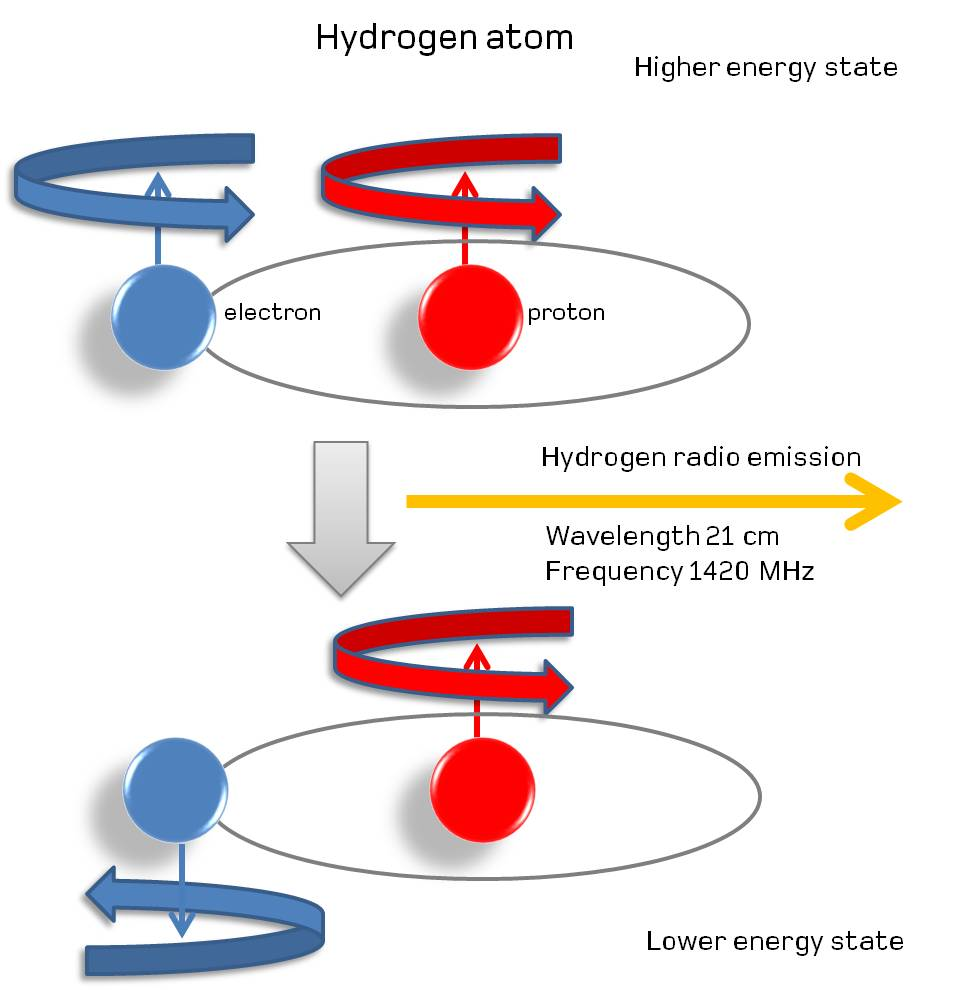
\includegraphics[width=0.5\linewidth]{Figures/Hydrogenemission1.jpeg}
		\caption{The formation of the \SI{21}{cm} wavelength line by the process of the spin flip transition where the hydrogen atom moves from one energy state to another. Image credit: {Square Kilometre Array}.}
		\label{Fig:21cm}
	\end{center}
\end{figure}

The populations of the low- and high-energy spin states, $n_0$ and $n_1$, define the spin temperature $T_s$:
\begin{equation}
\frac{n_0}{n_1} = \frac{g_1}{g_0}e^{(-E_10)/{k_B}{T_s}} = 3e^{{-T_*}{T_s}}.
\end{equation}
Here $\frac{g_1}{g_0}$ = 3 is the spin degeneracy of the triplet and singlet levels, and $T_{*}$ $\equiv$ $hc/k$ $\lambda_{21cm}$ = 0.068 K is the equivalent temperature of the hyperfine splitting of the two energy levels~\citep{2012RPPh...75h6901P}.

The \attention{globally averaged} brightness temperature $\delta$$T_b$ depends directly on $x_{HI}$, $z$, $T_S$, and $T_{CMB}$, but $T_S$ is heavily influenced by $T_K$ and the various coupling mechanisms. $x_{HI}$ is the fraction of neutral hydrogen \attention{[you define the neutral fraction in 2 places, and some of this text is redundant with the equation explanation below---condense where appropriate]}, the hydrogen spin temperature ($T_S$) is the excitation temperature of the 21 cm line, kinetic gas temperature, $T_K$, characterizes the thermal motion of atoms in the gas~\citep{2015aska.confE...1K,2006PhR...433..181F}. The equation	
\begin{equation}
\delta{T_b}\propto {x_{HI}}(1+z)^{1/2}({T_s}-{T_{CMB}})/{T_s}
\end{equation}
relates $\delta$$T_b$ to important factors which are \(x_{HI}\), the fraction of neutral hydrogen, redshift ($z$) and two temperatures, the spin temperature ($T_s$) and the CMB temperature ($T_{CMB}$).

Figure~\ref{Fig:epochs} describes the physical processes that are responsible for the frequency structures we see in the evolution of the sky-averaged 21 cm brightness temperature.

\begin{figure}
	\begin{center}
		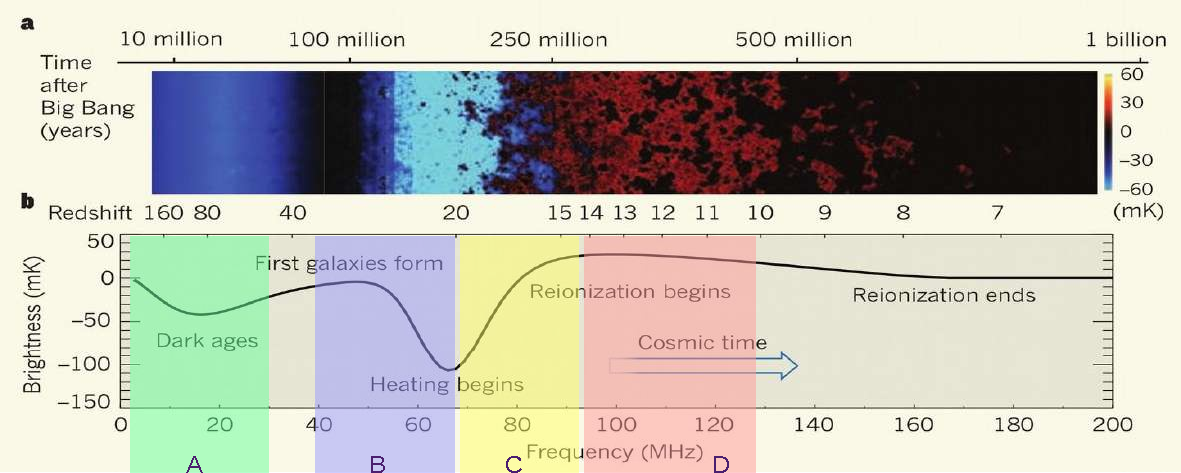
\includegraphics[width=\linewidth]{Figures/epo.pdf}\\
		\caption{Frequency structure of the globally averaged 21 cm signal: (a) shows the spatial and temporal evolution of the 21 cm brightness temperature and (b) shows the predicted time evolution of the globally averaged 21 cm brightness temperature ~\citep{2012RPPh...75h6901P}. There are different physical processes that govern the four highlighted (A to D) periods and the details are discussed in the main text.}			
		\label{Fig:epochs}
	\end{center}
\end{figure}

\subsection{Dark Ages}

The cosmic dark ages lie between recombination and cosmic dawn, beginning $\sim380,000$ years after the big bang and ending a few tens of million years later ($1100 > z > 30$),~\citep{2014arXiv1412.2096J} during which there were no luminous sources. The cosmic dark ages possess distinctive features that have never been explored to date. 

\textbf{Region A} in Figure~\ref{Fig:epochs} (green) highlights the dark ages period where the free electrons were no longer present. During this epoch, right after recombination, $T_K$=$T_\gamma$=$T_S$ where $T_\gamma$ is the temperature of the radiation background, typically set by the CMB so that $T_\gamma$ = $T_{CMB}$. During this period, matter that had separated from the CMB was cooled adiabatically as the universe expanded, which led to $T_K$ decreasing below $T_\gamma$~\citep{2006PhR...433..181F}. $T_S$ is initially coupled to $T_K$ as the collision between hydrogen atoms is effective at early times, resulting in $\delta T_b$ decreasing. As the universe expands and collisional coupling becomes ineffective, $T_S$ reverts to $T_\gamma$ because of CMB absorption, and $\delta T_b$ therefore eventually increases.

At this juncture, the most dominating matter in the universe was the dark matter and meager amounts of ordinary matter (neutral hydrogen and helium). After a few hundred million years, the dark and ordinary matter collapse together into halo-like structures through gravitational collapse, steadily cumulating physical matter and finally forming the first stars and galaxies, and that was the end of the cosmic dark ages~\citep{2003Sci...300.1904M}.

\subsection{Cosmic Dawn}

After the first stars' formation, their UV radiation couples to the HI line through the Wouthuysen-Field effect~\citep{2012RPPh...75h6901P}. Emission of Lyman Alpha photons by the first stars strongly couples $T_K$ and $T_S$ of the IGM; the described period is shown in \textbf{Region B} highlighted in purple. The coupling of $T_S$ to $T_K$ leads to a drastic absorption feature in $\delta T_b$. The absorption feature can be used to probe the formation processes of the first stars, with the potential of differentiating between Pop II and Pop III stars. \textbf{Region C} highlighted in yellow shows a period where the X-rays are emitted by hot accretion disks around the first stellar remnants (e.g., black holes) that effectively heat the cold HI gas. The heating of the neutral gas and constant coupling between $T_S$ and $T_K$ raised the overall spin-temperature to higher than the CMB temperature. Consequently, the 21-cm line became visible in emission at $z\sim15$. During radiation and heating, these first sources (possibly including mini-quasars) also ionized the gas around them, and a period of reionization started that is thought to have lasted until $z\sim5~to\sim 6$~\citep{2015aska.confE...1K}). The detailed $\delta T_b$ features are sensitive to the black hole properties and the progenitor's metallicity, offering further insight into first-star formation.~\citep{11}. \textbf{Region D} highlighted in red describes that when reionization begins, the neutral hydrogen supply is depleted ($x_{HI}$ decreases to zero), so $\delta T_b$ eventually also flatlines to zero because there is no more 21 cm signal left. 

\section{Hydrogen Line Observational Challenges}

Redshifted 21-cm radiation can penetrate dust and the Earth's atmosphere and is, therefore, an ideal tool for probing the history of the universe at any epoch of interest. However, ground-based telescopes and experiments are faced with several challenges when it comes to using the redshifted \SI{21}{cm} line emission to observe the dark ages, cosmic dawn, and the epoch of reionization. The primary challenges are human-made radio frequency interference (RFI), astrophysical foregrounds, ionospheric interference \attention{(the ionosphere is nearly opaque below 10~MHz)}, and instrumental systematics\st{, which is non-transparent below 10 MHz}. 

\subsection*{Brightness of Foreground Emission}

Foreground emission arises from both \attention{diffuse} Galactic \attention{structure} and extragalactic sources. The foreground emission's brightness temperatures are 4-5 orders of magnitude brighter than the cosmological \SI{21}{cm} signal. Galactic synchrotron emission is the primary foreground at low frequency and originates from the Galactic magnetic field's cosmic ray electrons' movement. Free electrons scattering off ions without being captured produces the Galactic free-free emission. The extragalactic foregrounds are predominantly radio-loud galaxies and quasars~\citep{2018RAA....18..114H, 2008MNRAS.389.1319J}.

\subsection*{Instrumental Systematics}\label{s:chall}

Global signal experiments measure total power and are therefore dominated entirely by systematics. \st{The faintness of the 21 cm signal presents a challenge as its characteristic scale is 0.1 mK. Few dipoles can be used to reach sensitivity.} \attention{[The point here is that 0.1 mK is actually ``easy'' to detect because it's ``bright.''  Replace the preceding text with the following sentence.]  The 21-cm absorption feature from cosmic dawn has a predicted amplitude of $\sim$0.1~mK.} To \st{include the order-of-magnitude} estimate \st{for} the amount of integration time needed to detect the cosmic dawn feature assuming statistical noise alone, \attention{we use the} \st{a} radiometer equation \st{is used, as follows},
\begin{equation}
T_{rms} = \frac{T_{sky}}{\sqrt{B. t_{obs}}},
\end{equation}
where $T_{rms}$ is the root mean square (rms) fluctuation of the sky temperature, $T_{sky}$ is the sky temperature, $B$ is the observation bandwidth, which can be varied, and $t_{obs}$ is the integration time in seconds. 
The required observing time can be estimated by
\begin{equation}
t_{obs} = \left ({\frac{T_{sky}}{T_{rms}}} \right )^2 \times \frac{1}{B}.
\end{equation}
For instance, $t_{obs}$ can be estimated to be \SI{3}{\hour} to reach the sensitivity of \SI{100}{\milli \kelvin} if $T_{rms} \sim 10 mK$, $T_{sky} \sim 1000 K$ and $B=$\SI{1}{\mega \hertz}. \st{Since the bandwidth can be varied, an integration time estimate of 1 day can be achieved. Though, the faintness of the 21 cm signal is a challenge, it can be alleviated with prolonged observations coupled with a large number of dipoles and/or a large effective area.} \attention{This calculation shows that statistical noise is typically not a limiting factor for cosmic dawn experiments.}

\subsection*{RFI}

Besides astrophysical challenges, human-made RFI saturates \st{the} \attention{manyfg
} frequency bands, increasing the need for isolated remote deployment sites. RFI can be orders of magnitude brighter than Galactic and extragalactic foregrounds. Unfortunately, RFI introduces a reduction in sensitivity in two separate but distinct ways: direct contamination by having similar spectral characteristics and overpowering the \SI{21}{\centi \meter} signal. The cosmic dawn signal \st{correlates} \attention{coincides} with the FM band (\SIrange{88}{108}{\mega \hertz} corresponding to 15$>$z$>$12), and FM contamination is especially predominant. Like radio transmitters that are run on the ground, satellite or aircraft communications often contribute to RFI. These RFI origins need not be nearby in many instances. Ionized meteor tracks, for example, are known to reflect RFI from remote areas. Inadequately shielded electronics can create self-generated RFI in the telescopes. RFI overpowers the signal from sources of astrophysical origin; therefore, mitigation must be applied. The foremost fundamental procedure for RFI mitigation is to prevent RFI in telescopes by deploying in remote areas. Other than site selection, there needs to be RFI removal during data analysis~\citep{2020PASP..132f2001L}. 

As much as RFI is challenging to avoid, there are a few restricted circumstances where it can be useful. The Orbcomm satellite transmission around \SIrange{137}{138}{\mega \hertz}, for instance, serves as a calibrator source that can be used to provide analytical mappings of an antenna's main beam patterns. With such satellites in low-Earth orbits that precede over time, these sources travel through the field of view of an antenna rapidly and regularly,  allowing a relatively densely sampled mapping of the primary beam~\citep{2015RaSc...50..614N, 2018PASA...35...45L}. 

\subsection*{Ionospheric Contamination}

The Earth's ionosphere also introduces significant fluctuations, which becomes increasingly refractive and turbulent below 100 MHz and becomes practically opaque below 10 MHz. In order to minimize RFI and ionospheric contamination, there have been proposals to observe long wavelengths from space-based telescopes further away from the ionosphere of our planet. These space-based telescopes do not exist yet, and there are several ground-based experimental efforts to understand how well we can make measurements from Earth~\citep{2019arXiv190710853C, 2019arXiv190804296K}. At night near-polar latitudes have lower plasma cutoff frequencies, and the cutoff is reduced during solar minima.

\section{Previous Cosmic Dawn and Low-frequency Experiments}

The \SI{21}{cm} wavelength of hydrogen gas is being observed by several experiments that are \st{modeled} \attention{designed} for Hydrogen mapping in our universe. Despite the challenges that are encountered in 21 cm cosmology, many experiments are nevertheless underway. This section highlights experiments aimed at frequencies corresponding to the dark ages ($1100 \lesssim z \lesssim 30$) and cosmic dawn ($30 \lesssim z \lesssim 10$).

\subsection{Global Signal Experiments for Cosmic Dawn}

The global signal experiments are most commonly located in remote RFI-quiet areas using single antennas with a large solid angle observing total power. However, there have been suggested and attempted innovative methods using interferometry. 

The Experiment to Detect the Global EoR Signature (EDGES) is located at Murchison Radio-astronomy Observatory (MRO) in Western Australia. The project's goal is radio detection of characteristic hydrogen signatures from cosmic dawn and the epoch of reionization. EDGES consists of a high-band instrument operating over the 90-200 MHz (14 $>$ z $>$ 6) range, a mid-band instrument operating over 60–160 MHz, and a low-band instrument that is sensitive to the 50-100 MHz (27 $>$ z $>$ 13) range~\citep{2017ApJ...835...49M}. 

The first detection of the 21 cm global signal was reported by \citet{2018Natur.555...67B} as a flattened absorption profile centered at a 78.1 MHz frequency, with an amplitude of 0.53 K and width of 18.7 MHz. \st{It} \attention{The amplitude} is more than a factor of two \attention{larger} \st{brighter} than the most optimistic model where no heating occurs until $z \sim$ 17, thus suggesting a hotter background or a colder than expected primordial gas.  \st{In terms of collisional dark matter}~\citet{2018Natur.555...71B, PhysRevD.98.103005} \st{and independent verification by similar experiments, the detection has called for an interpretation of newer physics.} \attention{The detection has spurred multiple interpretations of new physics, including collisional dark matter~\citep{2018Natur.555...71B, PhysRevD.98.103005}.  Independent verification by similar experiments is therefore of utmost importance.}

\st{EDGES experiment has been discussed, and the o}\attention{O}ther global signal experiments are summarised in Table~\ref{Tab:CD}. The included experiments are the Cosmic Twilight Polarimeter (CTP,~\citet{2019ApJ...883..126N}),  Large aperture Experiment to Detect the Dark Ages (LEDA,~\citet{2012JAI.....150004T, 2018MNRAS.478.4193P}), Mapper of the IGM Spin Temperature (MIST,~\citet{inproceedings}),   \prizm,~\citet{2019JAI.....850004P}, Radio Experiment for the Analysis of Cosmic Hydrogen (REACH,~\citet{8879199}), and the Shaped Antenna measurement of background RAdio Spectrum 2 (SARAS2,~\citet{2013ExA....36..319P})  

\begin{table}
	\centering
	\begin{tabular}{ c|ccc} 
		& Site & Frequency & Instrumental Approach \\
		\hline
		CTP & Troy, Virginia & 60--120 MHz & Dual-polarization Dipole \\
		
		LEDA & Owens Valley & 10--88 MHz & 251 Dual-polarization Dipoles \\
		
		MIST & MARS & 5--200 MHz & One Dipole Antenna \\
		\prizm\ & Marion Island & 30--200 MHz & 2 Dual-polarization Dipoles \\
		REACH & South African Karoo desert & 50--200 MHz & Monopole Antenna \\
		SARAS2 & Gauribidanur Obs., India & 87.5--175 MHz & Fat-dipole Antenna \\
		\hline
	\end{tabular}
	\caption{Active and upcoming global signal experiments. CTP, LEDA, MIST, \prizm\, REACH and SARAS 2 experiments with their deployment sites, frequency ranges and instrumental approach.}
	\label{Tab:CD}
\end{table}  

\subsection{Imaging below 30 MHz}

{\bf{Long Wavelength Astronomy Background}}

The father of radio astronomy, Karl G. Jansky, played a massive role in the inauguration of radio astronomy dating back to 1931. At that time, he was an employee at the Bell Telephone Laboratories as a radio engineer. Jansky was allocated to study and solve the problem that hindered the radio communication systems. Using highly directive antenna arrays shown in \autoref{Fig:Jansky}, he discovered that the static caused the radio frequency noise that hindered the communication systems from thunderstorms~\citep{book:BasicsofRA, book:RA}.

\begin{figure}
	\begin{center}
		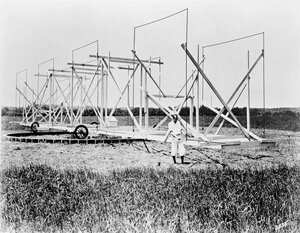
\includegraphics[width=0.7\linewidth]{Figures/jansky1.jpg}
		\caption{Jansky's highly directive antenna arrays which he used to discover the cause of RFI that hindered the communication systems at Bell Telephone Laboratories~\citep{book:BasicsofRA}}.
		\label{Fig:Jansky}
	\end{center}
\end{figure}

The antenna that he constructed operated at an approximated frequency of \SI{20}{MHz}, corresponding to an approximate long wavelength of \SI{15}{m}. He further found radio radiation from the Galactic Center at the operating frequency. Out of interest in Jansky's instigating discoveries, Grote Reber designed a radio telescope that operated at a range of approximately \SI{10}{MHz} to \SI{160}{MHz} (\SI{30}{m}-\SI{2}{m} wavelength) in 1937. He discovered that the \st{authoritative} \attention{dominant} source at longer wavelengths was the Milky Way. Furthermore, he realized that the radio telescope acts like a bolometer or a device to measure the heat. The antenna's radiation resistance measures an equivalent temperature of a distant part of space to which the 24 antenna response pattern projects it~\citep{1988JRASC..82...93R, CosmicStatic,2012PASP..124.1090H}.

Because of the research done for the communication systems, radio astronomy was born and expanded to radio astronomy and astrophysics~\citep{2012PASP..124.1090H}. The hydrogen line research area had an accelerated discovery, which was allocated an operating frequency of \SI{1420}{MHz} (\SI{21}{cm} wavelength) ~\citep{10.2307/530765}. After all these discoveries, the long-wavelength astronomy fascination has been resuscitated in the present epoch.

{\bf{Long Wavelength Astronomy Experiments}}

There are quite a few low-frequency experiments, but this document will briefly discuss a few measurements that exist at $\lessapprox$ 30 MHz. Two of these experiments represent the lowest frequencies measured to date (Reber's antenna, RAE-B). The other two represent the highest resolutions achieved in this frequency range (DRAO, OVRO-LWA).

Grote Reber constructed a state-of-the-art telescope operating at very low frequencies between 0.52 MHz and 2.1 MHz, which had 192 dipoles. At 2.1 MHz, the array had a resolution $\sim$ 5 \degree and was able to map the sky. The measurements were dominated by Galactic emission and the ionosphere as shown in Figure~\ref{Fig:Rebermap}~\citep{1988JRASC..82...93R}. 

\begin{figure}
	\centering
	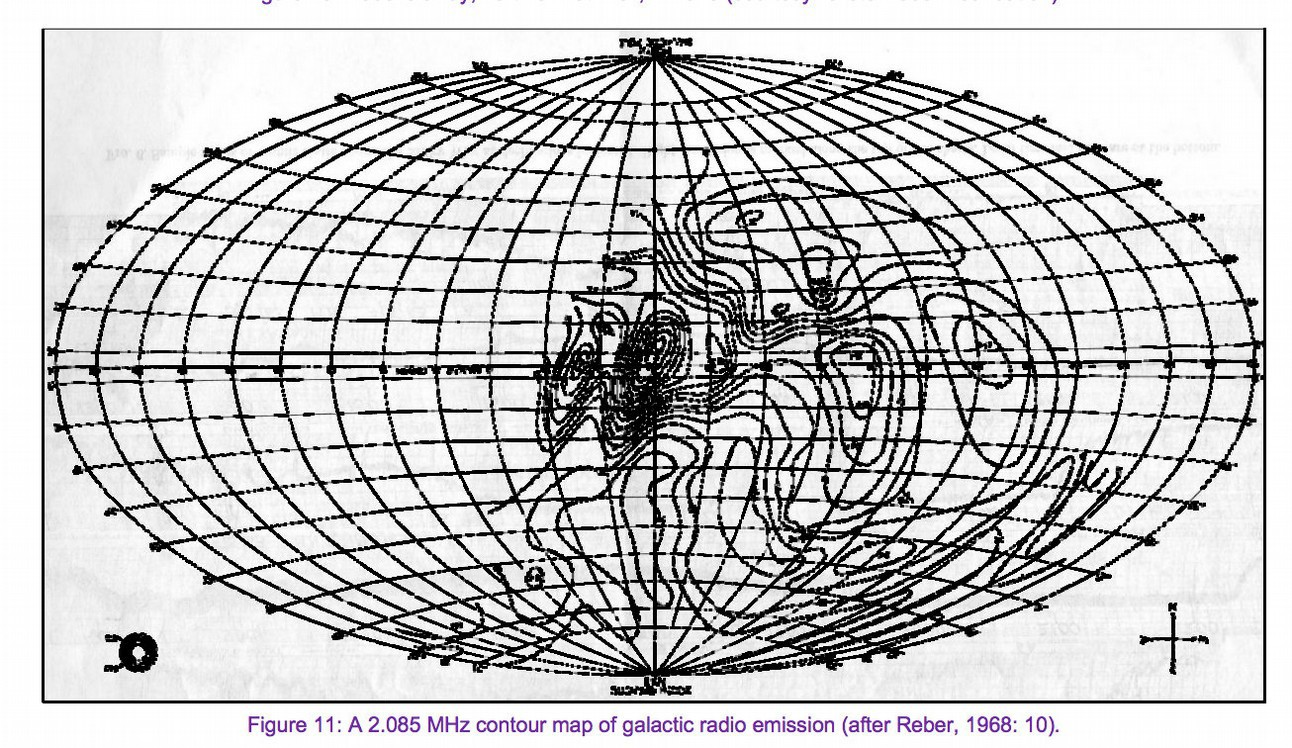
\includegraphics[width=0.7\linewidth]{Figures/Rebermap}
	\caption{Grote Reber's state-of-the-art map. The constructed array operated at very low frequencies between 0.52 MHz and 2.1 MHz and at 2.1 MHz, the array had a resolution of $\sim$ 5 \degree. It was able to map the sky, and the measurements were dominated by Galactic emission and the ionosphere~\citep{1988JRASC..82...93R}.}
	\label{Fig:Rebermap}
\end{figure}

The Radio Astronomy Explorer-2 (RAE-2) operated between 25 kHz and 13 MHz, with the primary science goal of radio measurements of our Galaxy, the Sun, Earth, and all the other planets. The resolution of this experiment is $\sim$10 \degree at \SI{4.7}{\mega\hertz}~\citep{1975A&A....40..365A}. \st{Thus far, the data presented is the only data that exists, and nothing exists elsewhere.}

Higher-resolution experiments include the OVRO-LWA, Dominion Radio Astrophysical Observatory (DRAO) 22 MHz telescope, and the DRAO \SI{10}{\mega\hertz} array. The OVRO-LWA operates at frequency ranges of \SI{36.528}{\mega\hertz} and \SI{73.152}{\mega\hertz}. At these frequencies, it has an angular resolution of \SI{15}{\arcminute}~\citep{2018AJ....156...32E}. The DRAO telescope operated at 22 MHz, and its resolution ranges between $\sim$1.1 \degree - 1.7 \degree. Its primary science goal was to measure the emission from discrete sources and observe our Galaxy's emission from its environment~\citep{1999A&AS..137....7R}. The DRAO 10 MHz array operated had a resolution of $\sim$ 2  \degree, and it was first used for discrete sources and was later used to map the large-scale structure of the background radiation~\citep{1976MNRAS.177..601C}.

\section{Structure of this Thesis}


The following is the outline of this thesis: in Chapter 2, 
Marion Island is introduced, the observing location of \prizm\ and \albatros. A summary of my voyage to Marion will also be provided. Chapter 3 will provide a full description of the \albatros\ instrument. Chapter 4 will provide a brief description of the \prizm\ instrument and present a summary of various system stages. In Chapter 5, preliminary results will be presented and conclude in the same chapter. My main contributions are listed below:
\begin{itemize}
	\item Designing a prototype solar power supply system in preparation for the 2019 Marion voyage, 
	\item Site inspection and installation of the first \albatros\ autonomous station at Marion Island in 2019,
	\item Helping with the revision and new designs of the \prizm\ subsystems, including the front end electronics enclosure, switch control circuit, 
	\item Designing the \prizm\ second stage electronics enclosure, which was in preparation for the 2020 deployment that did not happen.
\end{itemize}
